

\subsection{Baseline Methods}

To evaluate the performance of ACGNN in identifying cancer driver genes, we compared it against eight other methods. These included three state-of-the-art GCN-based approaches: EMOGI, MTGCN, and HGDC, which leverage multi-omics data as gene features and incorporate PPI networks to learn gene representations for cancer driver gene prediction. Additionally, we assessed five widely-used GNN methods: GCN~\cite{kipf2017semi}, GIN~\cite{xu2018powerful}, ChebNet~\cite{defferrard2016convolutional}, GraphSAGE~\cite{hamilton2017inductive}, and GAT~\cite{velickovic2018graph}, which are traditional graph neural network models that aggregate features from neighboring nodes and themselves in different manners to learn new representations. All methods, including ACGNN, were tested on three distinct PPI networks, using the same network structure and gene feature matrix \( X \in \mathbb{R}^{N \times 2048} \) as inputs. Here, \( N \) denotes the number of genes, and the pretrained embeddings are of dimension 2048, comprising four concatenated 256-dimensional bio-feature vectors (\( 256 + 256 + 256 + 256 \)) and a topological feature of dimension 1024. Details of the model architecture are provided in Table \ref{tab:model_arch}.

\subsection{Experiment Settings}

Our algorithm is implemented in Python 3.9, utilizing PyTorch 2.0.1 and PyTorch Geometric 2.3.1, within an environment that also includes DGL. The Adam optimizer is employed, and we use FocalLoss (\( \alpha = 0.25, \gamma = 2 \)) as the loss function. The learning rate is set to 0.001, with the number of training epochs fixed at 200 throughout all experiments, unless stated otherwise. All experiments were conducted on an Ubuntu server featuring an Intel CPU (2.4GHz, 128GB RAM) and an Nvidia RTX 4080 GPU. The time consumption and CPU/GPU usage for different methods are detailed in Table \ref{tab:consume_gpu}.


\subsection{Gene Embeddings Clustering}

The initial task performed using the obtained embeddings involved clustering the nodes within the gene association graph. The process began with dataset preparation and gene mapping, followed by configuring the model with specific parameters, such as the number of layers and embedding dimensions. During training, multiple epochs were executed, where each batch was processed by computing logits, calculating the loss using a binary cross-entropy function with class imbalance weighting, and updating model parameters through backpropagation using the Adam optimizer. After each epoch, validation was performed to evaluate model performance, and the best model was selected based on the validation loss.
Using the optimal model, the final node embeddings were generated, and cluster labels were assigned accordingly. These embeddings were further analyzed to extract cluster-specific insights, including the identification of significant nodes within each cluster. The final model state was saved to enable future use, providing a structured representation of the gene network through clustered node embeddings.
Figure~\ref{fig:heatmap_clustering} presents the hierarchical clustering of genes based on pretrained node embeddings of dimension 300. The heatmap visualizes gene expression patterns, with red and blue indicating high and low expression levels, respectively. 
The hierarchical clustering dendrograms at the top and left of the heatmap reveal distinct gene clusters, highlighting structural similarities among genes. The presence of highly correlated gene groups suggests that the embedding model effectively captures biologically meaningful relationships.
Notably, genes such as \textit{NUP37}, \textit{CD2AP}, and \textit{AKT1} form distinct subclusters, implying potential functional similarity or co-regulation. In contrast, genes like \textit{EGFR}, \textit{ATR}, and \textit{STAT3} are grouped in separate regions, potentially reflecting their involvement in distinct biological pathways.
The structure of the heatmap demonstrates that the pretrained embeddings provide an informative representation of gene features, facilitating downstream analyses such as functional enrichment and pathway analysis.


\begin{figure}
	\centering
	\scriptsize
	\captionsetup{font=scriptsize}
	%\captionsetup{font=footnotesize}
	%%\captionsetup{font=scriptsize}
	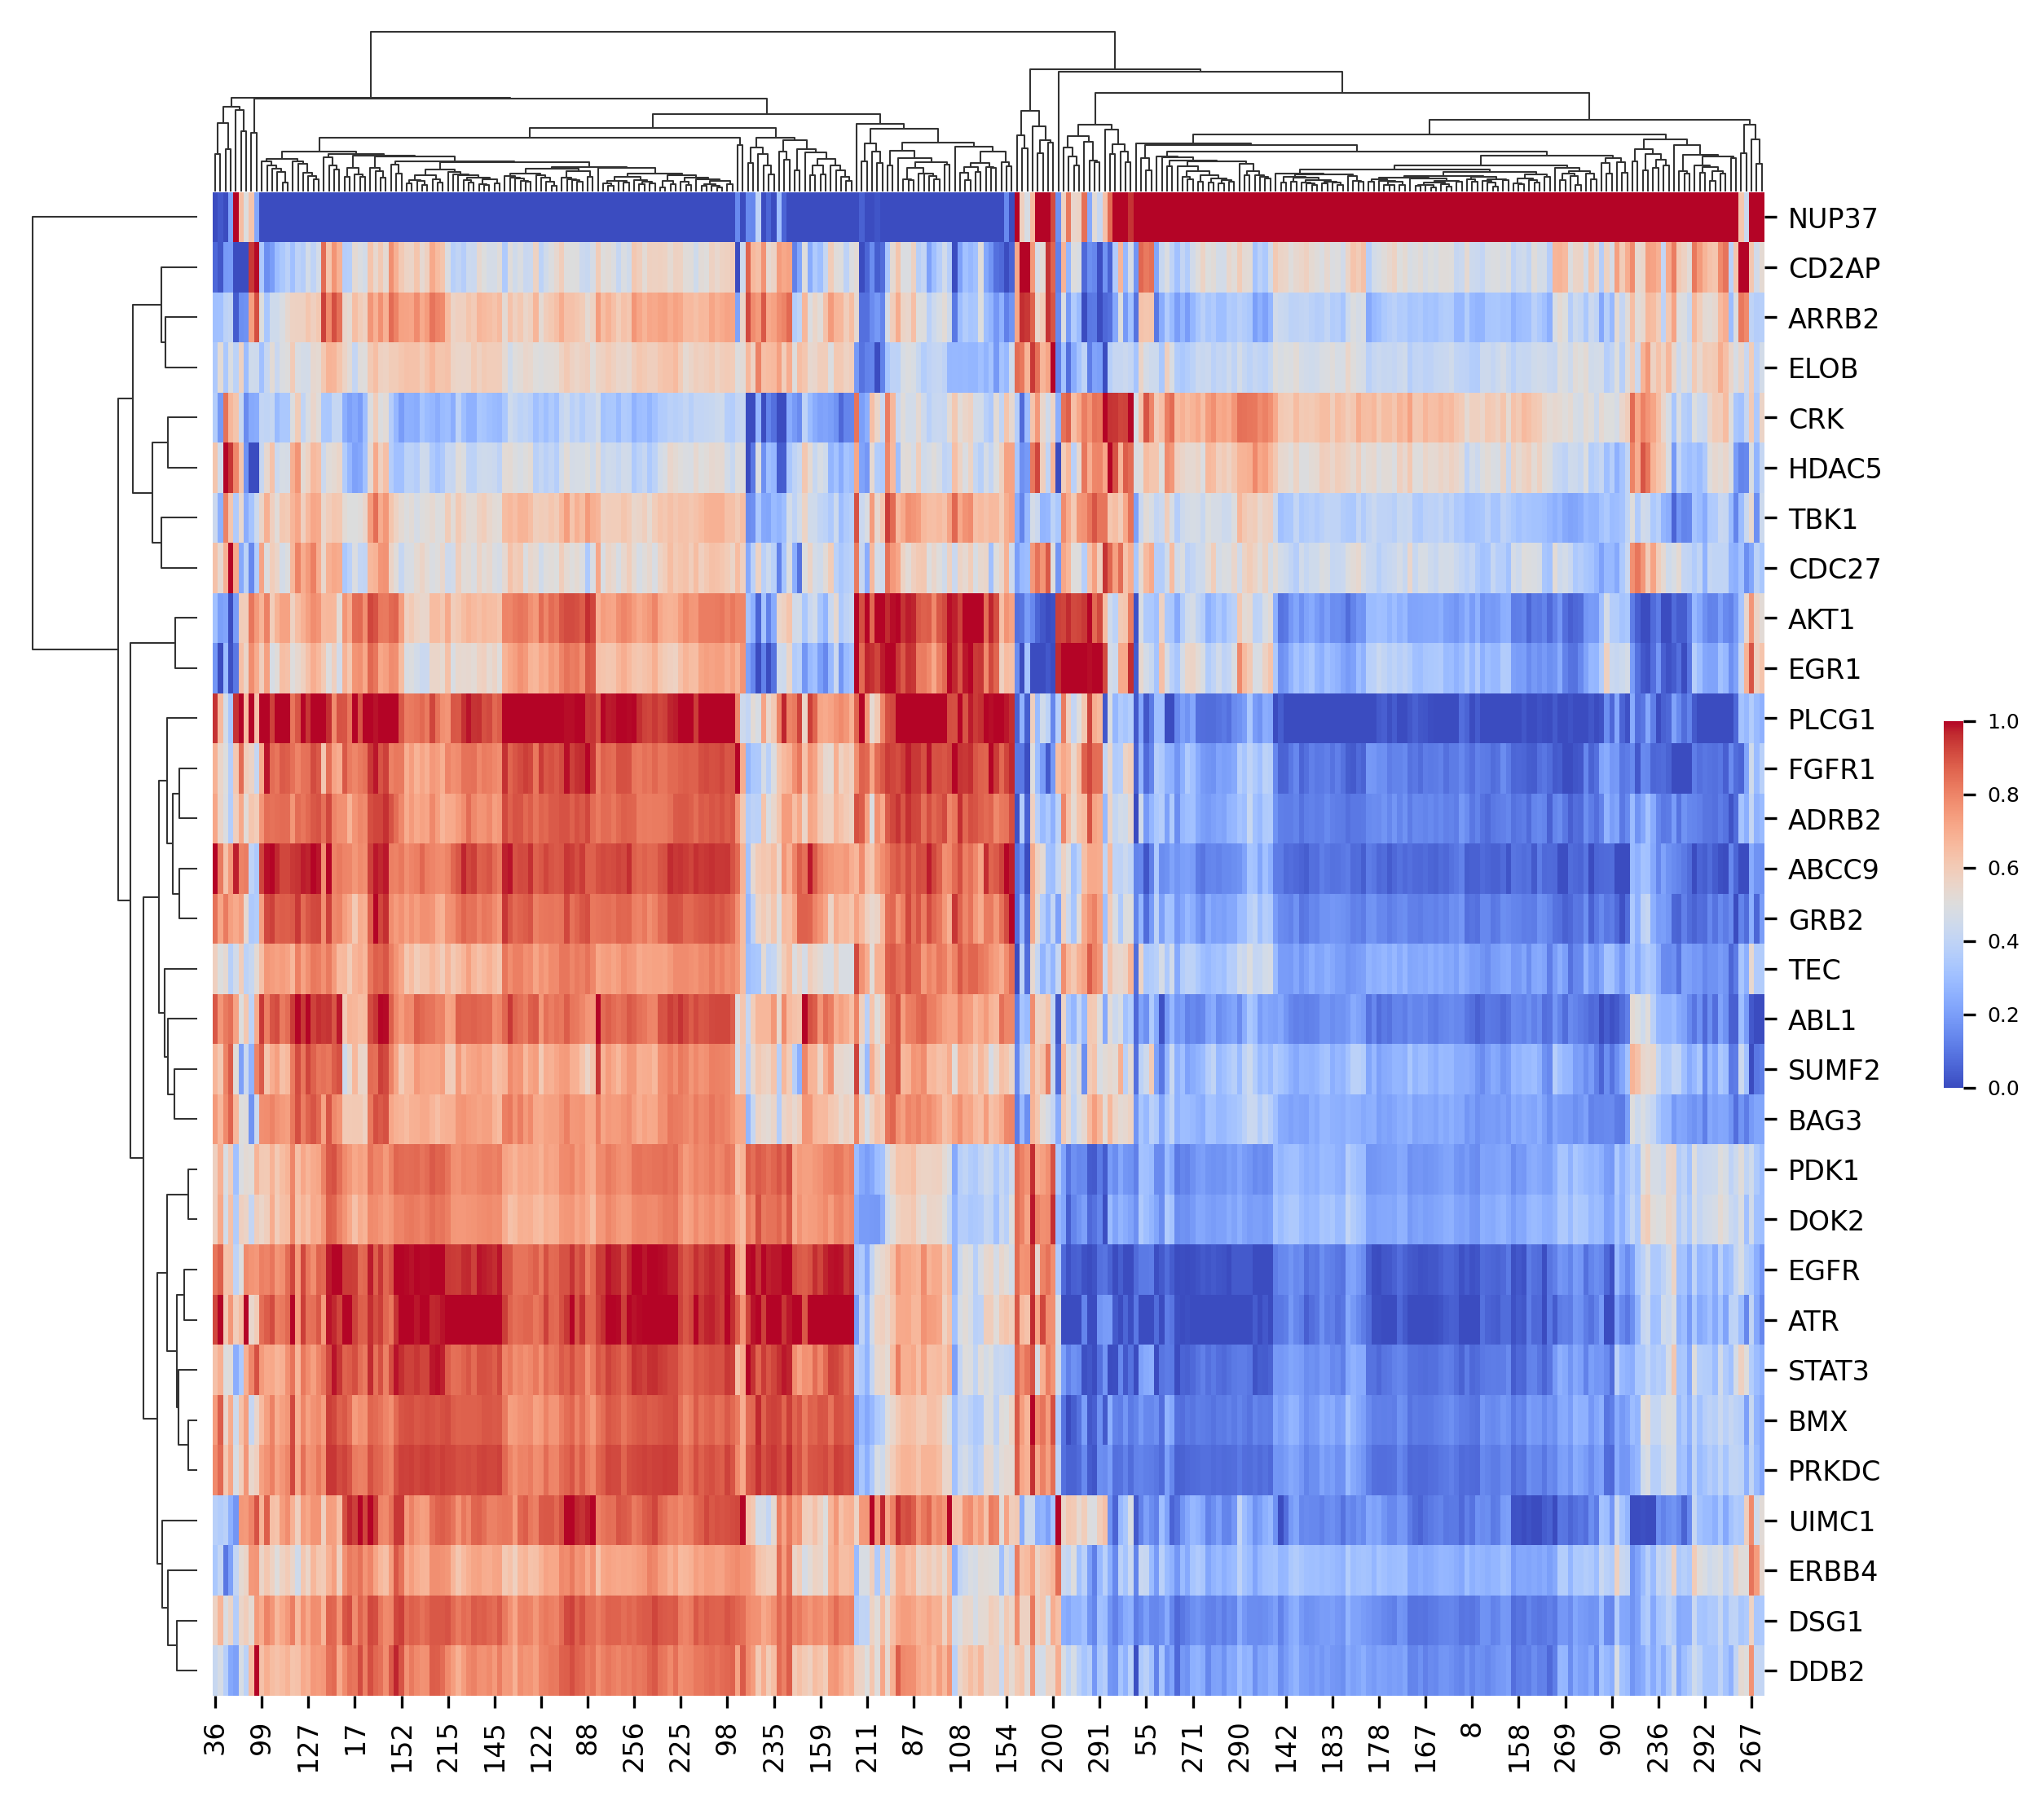
\includegraphics[width=0.49\textwidth]{images/KIRP_embeddings_matrix_stId_head2_dim16_lay2_epo100_.png}
	\caption{Demonstration of pretrained node embeddings with a dimension of 300 for clustering genes into k=30 clusters.}
	\label{fig:heatmap_clustering}
\end{figure}



%\vspace{0.5cm} % Adjust the space as needed 
\begin{figure}
	\centering
	%\captionsetup{font=scriptsize}
	\scriptsize
	%\captionsetup{font=scriptsize}
	\captionsetup{font=footnotesize}
	\subfloat[CPDB]{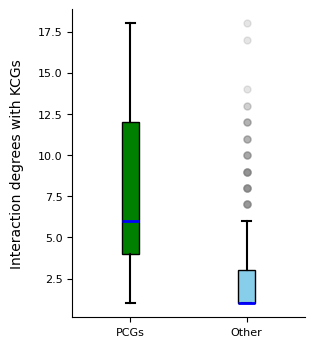
\includegraphics[width=1.2in]{images/__ACGNN_CPDB_degree_distributions_epo103_2048.png}}  
	\subfloat[STRING]{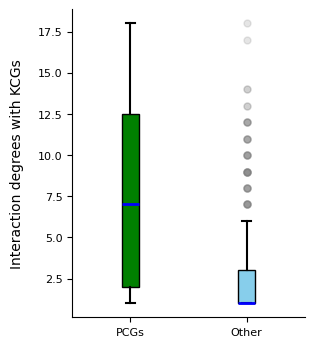
\includegraphics[width=1.2in]{images/__ACGNN_STRING_degree_distributions_epo103_2048.png}}
	\subfloat[HIPPIE]{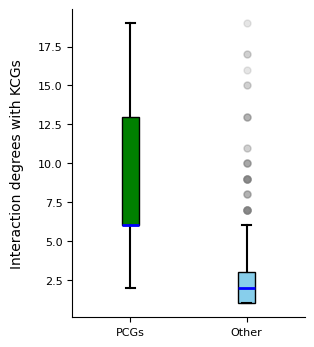
\includegraphics[width=1.2in]{images/__ACGNN_HIPPIE_degree_distributions_epo103_2048.png}}\\    
	\caption{The interaction distributions of Predicted Cancer Genes (PCGs) with Known Cancer Genes (KCGs) across three different protein-protein interaction (PPI) networks: CPDB, STRING, and HIPPIE.}
	\label{fig:degree}
\end{figure}

%\bigskip

\vspace{0.5cm} % Adjust the space as needed 
\begin{figure*}
	\centering
	%\captionsetup{font=scriptsize}
	\scriptsize
	%\captionsetup{font=scriptsize}
	\captionsetup{font=footnotesize}
	\subfloat[CPDB]{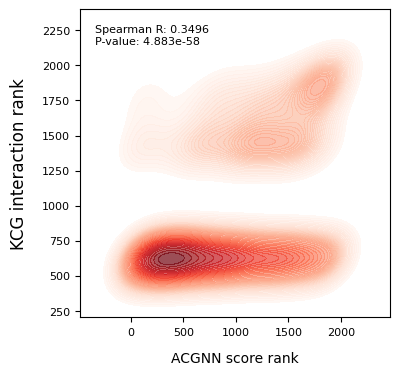
\includegraphics[width=2.0in]{images/CPDB_kde_plot_epo101_2048.png}}  
	\subfloat[STRING]{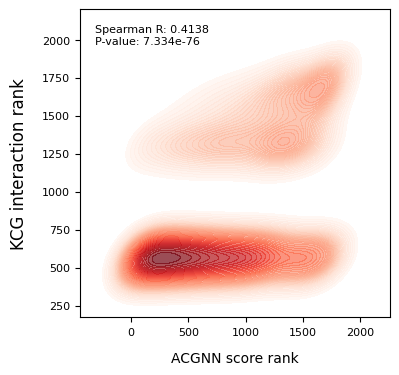
\includegraphics[width=2.0in]{images/STRING_kde_plot_epo101_2048.png}}
	\subfloat[HIPPIE]{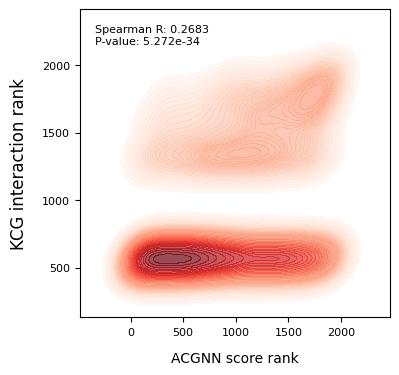
\includegraphics[width=2.0in]{images/HIPPIE_kde_plot_epo101_2048.png}}\\    
	\caption{Kernel Density Estimation (KDE) plot illustrating the distribution of interaction degrees for predicted driver genes and other genes. The x-axis represents the inteaction degree, and the y-axis represents the density.}
	\label{fig:kde_plot}
\end{figure*}


\begin{figure}[ht]
	\centering
	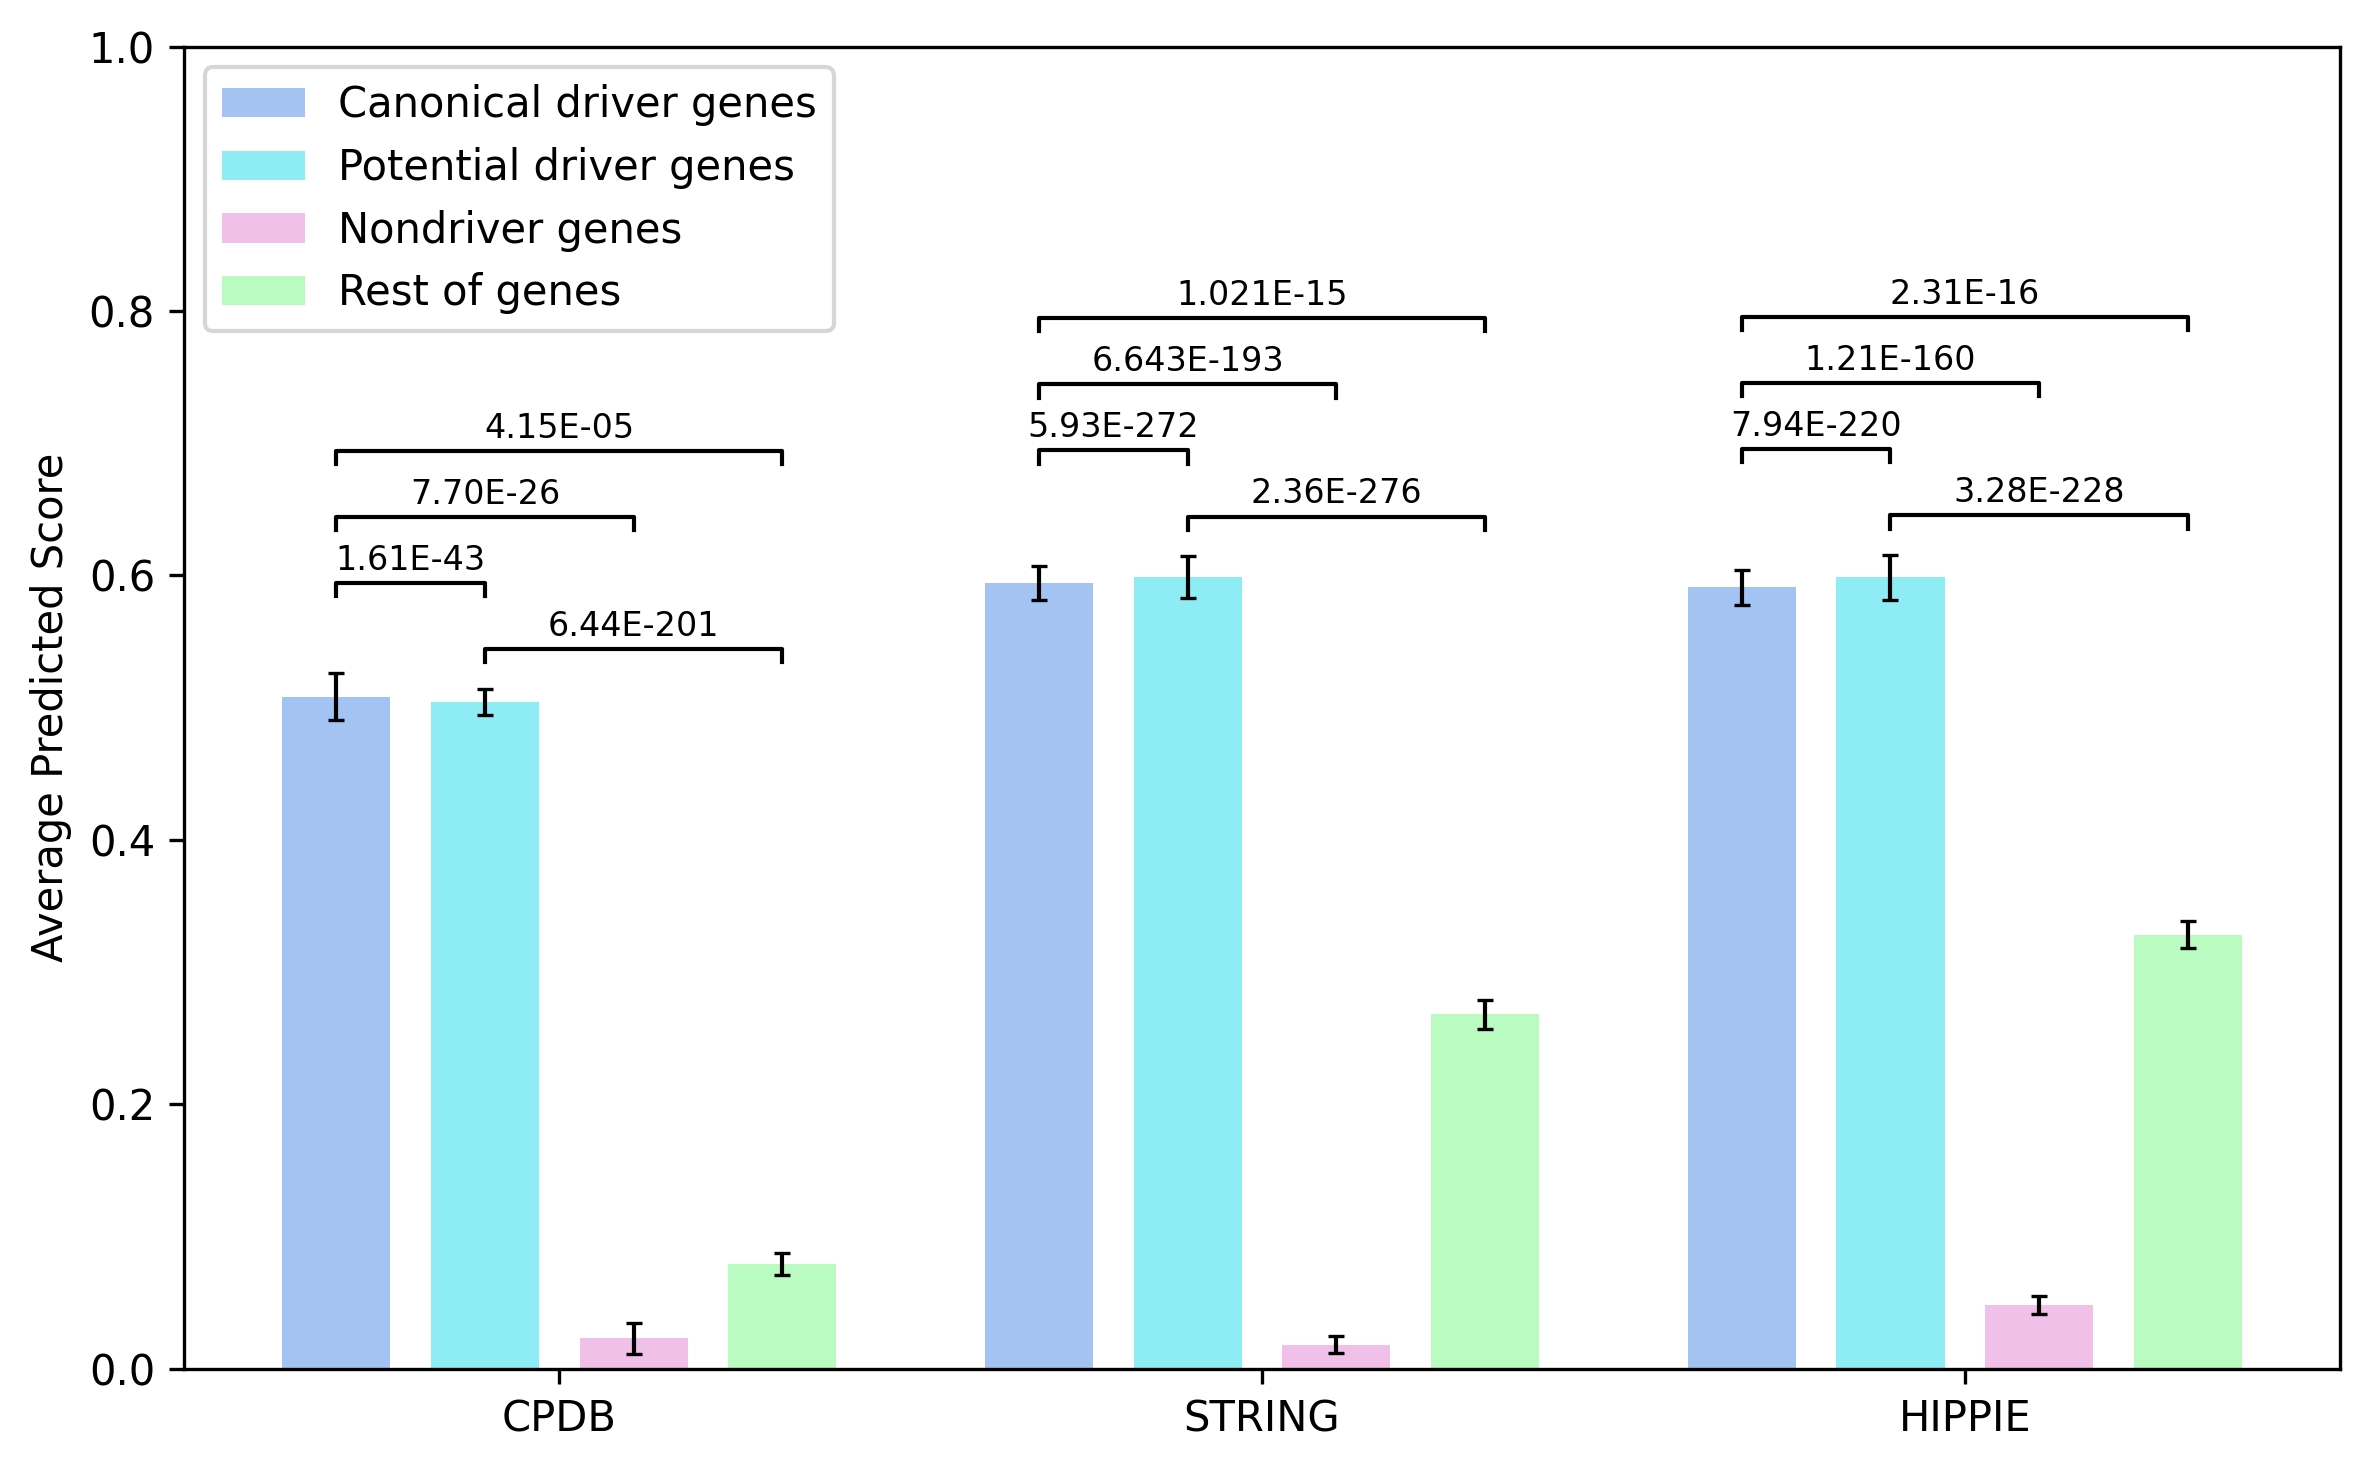
\includegraphics[width=0.45\textwidth]{images/average_predicted_scores.png}
	\captionsetup{font=footnotesize}
	\caption{Average predicted scores for different networks and gene types. The bar plot displays the scaled predicted scores for canonical driver genes, potential driver genes, nondriver genes, and the rest of the genes across three biological networks: CPDB, STRING, and HIPPIE. Error bars represent the scaled standard errors of the mean (SEM). The statistical significance (p-values) for comparisons between gene categories within each network is annotated above the bars. Numbers above the brackets represent the p-values of the Spearman Rank Correlation Test, indicating the significance of differences between groups.}
	
	\label{fig:predicted_scores}
\end{figure}


\begin{figure}[ht]
	\centering
		\scriptsize
	%\captionsetup{font=scriptsize}
	\captionsetup{font=footnotesize}
	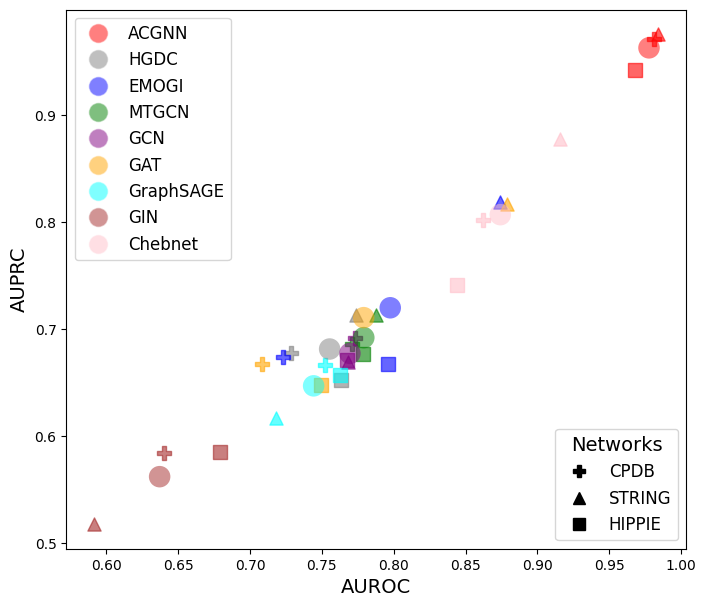
\includegraphics[width=0.45\textwidth]{images/roc_pr.png}
	\caption{
		Performance comparison of graph-based models across different biological networks. 
		The scatter plot shows the area under the receiver operating characteristic curve (AUROC) on the x-axis and the area under the precision-recall curve (AUPRC) on the y-axis for various models. The large circles represent the mean AUC values across biomolecular networks for each method.
	}
	\label{fig:auroc_auprc_comparison}
\end{figure}


\begin{figure}[ht]
	\centering
		\scriptsize
	%\captionsetup{font=scriptsize}
	\captionsetup{font=footnotesize}
	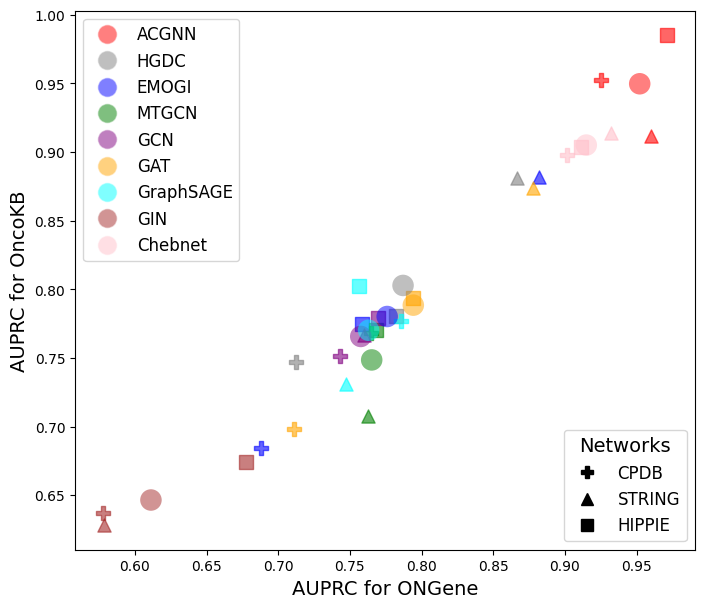
\includegraphics[width=0.45 \textwidth]{images/__comp_oncokb_ongene_acgnn.png}
	\caption{Performance comparisons of different methods on biomolecular networks. Results of all methods were evaluated on two independent test sets derived from the OncoKB and ONGene databases, respectively. The large circles represent the mean AUPRC values across biomolecular networks for each method.}
	\label{fig11}
\end{figure}



\subsection{Performance on Driver Gene Prediction}
We evaluated our method and baseline approaches for predicting driver genes on pan-cancer multi-omics dataset, using the average AUROC and AUPRC from ten iterations of validation as performance metrics. \noindent Table~\ref{tab:model_arch} presents the architectural details of different models used in our study. ACGNN stands out with the highest parameter count of 7,346,177, attributed to its deeper architecture with five layers. In contrast, most baseline models, including HGDC, EMOGI, MTGCN, GCN, GAT, and GraphSAGE, employ a three-layer structure with a comparable number of parameters, ranging from approximately 4.19M to 4.20M. Notably, GraphSAGE has a higher parameter count of 7,344,129, indicating increased complexity despite having the same number of layers as the other baselines. GIN follows with 6,297,601 parameters, showing a moderate increase in complexity. ChebNet exhibits the highest parameter count of 10,489,857, highlighting its expressive power but also potential computational overhead. These architectural differences contribute to variations in model performance, as analyzed in the subsequent sections. 
Figure~\ref{fig:auroc_auprc_comparison} presents the performance of various graph-based models on different biological networks. The x-axis represents the AUROC values, which indicate the classification ability of each model, while the y-axis represents the AUPRC values, highlighting precision-recall performance.
From the plot, ACGNN achieves the highest AUROC and AUPRC, demonstrating strong predictive performance. HGDC, EMOGI, and MTGCN show competitive results, clustering around an AUROC of 0.75–0.85. The choice of biomolecular networks (CPDB, STRING, HIPPIE) influences model performance, as reflected in the varied shapes. GCN, GAT, and GraphSAGE exhibit moderate results, suggesting their dependency on network topology.
Table~\ref{tab:roc_pr} presents the average performance of ACGNN and eight other methods across different biomolecular networks. ACGNN consistently achieves the highest performance, particularly excelling in CPDB and STRING. ChebNet also performs strongly, especially in STRING and HIPPIE. In contrast, GIN and GraphSAGE tend to underperform across multiple datasets, highlighting their limitations in certain network structures.

 Figure~\ref{fig11} compares the AUPRC performance of various methods across different biological networks using independent test sets from OncoKB and ONGene. The x-axis represents the AUPRC for ONGene, while the y-axis represents the AUPRC for OncoKB. 
ACGNN continues to outperform other models, achieving the highest scores across both test sets. HGDC, EMOGI, and MTGCN display competitive results, clustering between 0.75 and 0.85 AUPRC. The distribution of models across CPDB, STRING, and HIPPIE networks indicates variations in predictive performance due to differences in biological network structures.
The results demonstrate that methods leveraging advanced GNN architectures, particularly ACGNN, provide superior predictions in cancer driver gene identification compared to traditional models.


Figure~\ref{fig:degree} presents the interaction distributions of Predicted Cancer Genes (PCGs) with Known Cancer Genes (KCGs) across three different protein-protein interaction (PPI) networks: CPDB, STRING, and HIPPIE. The boxplots illustrate the interaction degrees between these gene categories, offering insights into their connectivity patterns.
In the CPDB network (Figure~\ref{fig:degree} a), PCGs exhibit a wider distribution of interaction degrees, with a higher median and several outliers. This suggests that PCGs in CPDB tend to have stronger connectivity with KCGs. The STRING network (Figure~\ref{fig:degree} b) follows a similar pattern, though with slightly lower median values and fewer extreme outliers, indicating a moderate connectivity between PCGs and KCGs. The HIPPIE network (Figure~\ref{fig:degree} c) displays the highest median interaction degree among the three networks, suggesting that it might capture a denser set of biologically relevant interactions for PCGs.
Across all three networks, PCGs demonstrate significantly higher interaction degrees with KCGs compared to other genes. The interquartile range (IQR) and median values for PCGs are consistently larger, while the presence of multiple outliers suggests that some PCGs have exceptionally high connectivity with KCGs. In contrast, the Other gene category has a much lower and more compact distribution, indicating weaker associations with KCGs.
These results reinforce the relevance of PCGs in cancer research, as their strong connectivity with known cancer genes suggests potential biological significance. The differences observed across the three networks highlight the impact of network-specific interaction curation, with HIPPIE capturing the densest set of interactions. 

Kernel Density Estimation (KDE) (Figure~\ref{fig:kde_plot}) presents the average predicted scores for different gene types across the three biological networks. The bar plot categorizes genes into canonical driver genes, potential driver genes, nondriver genes, and the rest of the genes. The error bars represent the scaled standard errors of the mean (SEM), ensuring statistical robustness in the displayed values.
Across all three networks, canonical driver genes consistently exhibit the highest predicted scores, followed by potential driver genes, while nondriver genes and the rest of the genes have significantly lower scores. This pattern suggests a strong alignment between the model’s predictions and known biological classifications of driver genes.
The statistical significance of the differences in predicted scores is annotated above the bars, with p-values from the Spearman Rank Correlation Test. The highly significant p-values (e.g., \( p < 10^{-40} \) in CPDB and similar magnitudes in STRING and HIPPIE) indicate strong differentiation between gene categories, reinforcing the predictive power of the model in distinguishing cancer-related genes.
Additionally, STRING and HIPPIE networks exhibit a greater separation between gene categories than CPDB, suggesting that these networks may capture more biologically relevant interactions. The increased predicted scores for the "rest of the genes" category in HIPPIE compared to CPDB and STRING could indicate a broader connectivity pattern in HIPPIE's network structure.
These results highlight the model’s ability to predict meaningful biological classifications across different interaction networks, with STRING and HIPPIE demonstrating particularly strong discriminatory power.


	

\subsection{Performance on OncoKB and ONGene}
To investigate whether the models’ performance is biased toward a specific dataset, we evaluated them on two additional cancer gene databases: OncoKB~\cite{chakravarty2017oncokb} and ONGene~\cite{liu2017ongene}. The cancer gene sets from OncoKB and ONGene are compiled from scientific literature or clinical studies and are therefore not explicitly informed by any of the data types used to train ACGNN . This demonstrates ACGNN 's capability to predict cancer genes broadly, independent of the methods or data used to define them, across the Gene Network, Pathway Network, and Protein-Protein Interaction Network. For this evaluation, the test set was masked exclusively for non-labeled genes.

The performance comparisons of different methods across biomolecular networks are illustrated in Figure~\ref{fig11}. A clear positive correlation between AUPRC values for the ONGene and OncoKB datasets is observed, indicating that methods performing well on one dataset tend to perform well on the other. This highlights the robustness and generalizability of certain methods across diverse, independent cancer gene sets.
Among the evaluated methods, ACGNN  achieves the highest performance on both datasets, as reflected by its red markers clustered near the top-right corner of the plot. Furthermore, ACGNN  maintains consistently high average AUPRC values, underscoring its reliability in network-based cancer gene prediction tasks.
These results emphasize the critical importance of integrating multiple biomolecular networks and leveraging advanced graph-based models for accurately identifying cancer driver genes. The alignment between the results from the OncoKB and ONGene datasets further validates the relevance and applicability of these methods in advancing cancer research.
 


\subsection{Feature Ablation Experiment}

The feature ablation experiments provide insights into the influence of different multi-omics data and biomolecular networks on the performance of ACGNN, as shown in Table \ref{tab:roc_pr_ablate}.
The table presents the ablation study results for different network variants trained on three biological networks: CPDB, STRING, and HIPPIE. The models tested include ACGNN, AC256x1, AC256x2, AC256x4, and AC1024x1. 
 ACGNN, the full model incorporating all bio-features and topological information, achieves the highest AUROC and AUPRC across all networks, demonstrating the advantage of integrating comprehensive features. AC256x1, using only one type of biological feature, and AC256x2, utilizing two types, show a decline in performance, indicating that limited biological features reduce predictive power. AC256x4, incorporating four types of biological features, performs better than AC256x2, suggesting that more bio-features enhance model performance. AC1024x1, which relies solely on topological information, has the lowest AUROC and AUPRC scores across most networks, confirming the critical role of biological features. These results highlight that incorporating multiple biological features significantly improves predictive accuracy, with the best performance achieved when combining all bio-features with topological information in ACGNN.

 
\subsection{Evaluation of Cancer Type-Specific Driver Gene Prediction}

We also investigate the effectiveness of ACGNN in detecting driver genes of a single cancer type. The results in Table \ref{tab:cancer_results} presents the AUROC (Area Under the Receiver Operating Characteristic Curve) and AUPRC (Area Under the Precision-Recall Curve) scores for various cancer types using four different methods: HGDC, EMOGI, MTGCN, and ACGNN. These metrics assess the predictive performance of each model across three feature types: biological (Bio), topological (Topo), and combined (Comb).
ACGNN consistently outperforms the other methods across all cancer types. The bolded values in the table indicate that ACGNN achieves the highest AUROC and AUPRC scores in nearly all cases, highlighting its effectiveness in predicting miRNA-disease associations compared to HGDC, EMOGI, and MTGCN. For instance, in bladder cancer (BLCA), ACGNN with combined features achieves an AUROC of 0.9644 and an AUPRC of 0.9766, significantly surpassing the next best method, MTGCN (Comb), which records an AUROC of 0.7525 and an AUPRC of 0.8174.

The integration of biological and topological features (Comb) consistently yields the best performance across all cancer types. In most cases, the AUROC and AUPRC values for the combined feature type are the highest, indicating that incorporating both biological and topological information enhances predictive accuracy. For example, in liver cancer (LIHC), ACGNN with combined features achieves an AUROC of 0.9704 and an AUPRC of 0.9809, outperforming the biological-only (AUROC = 0.9073, AUPRC = 0.9391) and topological-only (AUROC = 0.8513, AUPRC = 0.9022) configurations.
Certain methods exhibit limitations with specific cancer types. HGDC consistently performs the worst, frequently yielding the lowest AUROC and AUPRC values. While EMOGI and MTGCN produce competitive results in some cases, they are generally outperformed by ACGNN. For instance, in cervical cancer (CESC), HGDC with topological features achieves an AUROC of 0.6635 and an AUPRC of 0.7085, considerably lower than ACGNN with combined features, which attains an AUROC of 0.9760 and an AUPRC of 0.9871.
The superior performance of ACGNN across multiple cancer types suggests strong generalizability. 

 
  \subsection{Prediction of Novel Cancer Driver Genes}
  \noindent In this section, we investigate the performance of ACGNN in identifying novel cancer genes across three biomolecular networks: CPDB, STRING, and HIPPIE. The CPDB network consists of 5,693 nodes and 31,761 edges, while STRING contains 10,430 nodes and 58,559 edges. HIPPIE, the largest of the three, comprises 12,981 nodes and 84,969 edges. These networks provide diverse interaction patterns, enabling a comprehensive evaluation of ACGNN’s predictive capabilities.
  
  \noindent To evaluate the performance of ACGNN across different biomolecular networks, we computed the predicted scores for various gene categories, including canonical driver genes (CDGs), nondriver genes, potential cancer genes curated in the NCG 6.0 database, and other genes. The analysis was conducted across three biomolecular networks: CPDB, STRING, and HIPPIE. The results provide insights into how ACGNN distinguishes between different gene types within these networks, highlighting its capability to identify potential cancer-associated genes with high confidence.
 
  \noindent Figure~\ref{fig:predicted_scores} illustrates the average predicted scores of different gene categories (canonical driver genes, potential driver genes, nondriver genes, and the rest of genes) across three biomolecular networks: CPDB, STRING, and HIPPIE. The results indicate that canonical and potential driver genes consistently achieve significantly higher predicted scores compared to nondriver genes and the rest of the genes, suggesting strong model confidence in identifying cancer-associated genes. The statistical significance between different gene categories is denoted by p-values, all of which are extremely small, confirming the robustness of the model's predictions. Notably, the predicted scores of canonical and potential driver genes exhibit minimal variance, further reinforcing the model’s reliability across diverse biomolecular networks. The STRING and HIPPIE networks show slightly higher predicted scores for driver genes compared to CPDB, indicating that these networks might provide more informative gene interactions for the model.
  
To identify novel cancer driver genes, we trained the model using the CPDB network on the full training dataset with 500 epochs. Predictions were filtered by applying a threshold of 0.99, ensuring that only potential cancer driver genes were included while excluding previously labeled genes. This process resulted in 352 predicted cancer driver genes, of which 55 are already known cancer drivers. Additionally, 204 of the novel predictions have at least one supporting piece of evidence suggesting their potential as cancer drivers, based on sources such as NCG’s candidate cancer genes \cite{Repana2019}, OncoKB’s manually curated cancer genes, ONGene’s literature-curated cancer genes, and IntOGen's catalog of cancer-related mutations \cite{martinez2020compendium}. Among the top 60 predicted novel driver genes, 71.67\% (43 out of 60) have at least one supporting source indicating their potential role in cancer (Table \ref{table:gene_sources}).
 
 	\begin{table*}[h]
 	\centering
 	\begin{tabular}{llllll}
 		\toprule
 		\textbf{Gene} & \textbf{Confirmed Sources} & \textbf{Gene} & \textbf{Confirmed Sources} & \textbf{Gene} & \textbf{Confirmed Sources} \\
 		\midrule
 		ACTB & OncoKB, NCG, IntOGen & VDAC1 &  & SRP68 & IntOGen \\
 		CXCL2 & OnGene & BMP1 & IntOGen & CHMP6 &  \\
 		TRAF2 & OncoKB, NCG, IntOGen & CDK2 &  & DDB1 & IntOGen \\
 		RBBP4 & IntOGen & CRKL & OncoKB, OnGene & FHL2 & OnGene \\
 		UBC & IntOGen & KAT2B &  & HCK & IntOGen \\
 		LIN37 &  & ATR & OncoKB, NCG, IntOGen & ZWINT & NCG \\
 		FREM2 & NCG, IntOGen & CHRD & IntOGen & ACTN2 & IntOGen \\
 		LEF1 & OncoKB, OnGene, NCG, IntOGen & SIAE &  & DAXX & OncoKB, OnGene, NCG, IntOGen \\
 		PEX5 &  & UBXN7 & NCG & TEAD4 & IntOGen \\
 		ORC5 &  & TPM3 & OncoKB, NCG & RBM39 & NCG, IntOGen \\
 		NFKB1 & IntOGen & ABHD5 &  & HDAC1 & OncoKB, OnGene, NCG \\
 		HDAC2 & OncoKB, NCG & BIRC2 & OnGene & GRB2 & NCG, IntOGen \\
 		FOXK1 & NCG & GAB1 & OncoKB & EGFR & OncoKB, OnGene, NCG, IntOGen \\
 		PURA &  & TPM1 &  & KAT5 &  \\
 		HDAC3 & IntOGen & RBL1 & IntOGen & ATF5 & IntOGen \\
 		PRKDC & OncoKB, NCG, IntOGen & CDK9 &  & MYOM1 & IntOGen \\
 		NUP37 &  & TBP & NCG, IntOGen & ERCC6 & NCG, IntOGen \\
 		CDC20 & NCG & TBCA &  & GNA13 & OncoKB, OnGene, NCG, IntOGen \\
 		CASP7 &  & PLK1 & OnGene, NCG, IntOGen & SF3B3 & NCG \\
 		TRAF6 & OnGene, NCG, IntOGen & HDHD3 & IntOGen & UBE2B &  \\
 		\bottomrule
 	\end{tabular}
\caption{The top 60 predicted driver genes along with their confirmed sources, with unconfirmed genes left blank. Among these, 71.67\% of the novel genes have at least one supporting piece of evidence indicating their potential as cancer drivers. In total, 43 out of 60 genes are confirmed.}
 	\label{table:gene_sources}
 \end{table*}
 
 